%\documentclass[journal]{IEEEtran}
%\documentclass[12pt,onecolumn]{IEEEtran}
\documentclass[UTF8]{article}
\usepackage{ctex}
\usepackage{geometry,graphicx,marvosym}
\usepackage{amsmath,amsthm}
\usepackage{amsfonts}
\usepackage[usenames,dvipsnames]{pstricks}
\usepackage{pst-plot,pstricks-add}
%\usepackage{graphicx,times,amsmath,amssymb,multirow,subfigure}
\usepackage{graphicx,times,amsmath,amssymb,multirow}
\usepackage{url}
\usepackage{stfloats}
\usepackage{amsfonts,rotating}
\usepackage{color}
\usepackage{verbatim,multirow}
% setting dimension of the paper
\textwidth 7.0true in
\textheight 8.9 true in
\topmargin=-20pt
\headheight=6pt
\headsep=2pt
\oddsidemargin -0.3true in
\evensidemargin -0.4true in
\usepackage{amssymb}

\newtheorem{theorem}{Theorem}
\newtheorem{lemma}{Lemma}
\newtheorem{algorithm}{Algorithm}
\newtheorem{definition}{Definition}
\newtheorem{proposition}{Proposition}

\newcommand{\dtcwt}{\operatorname{DT-\mathbb{C}WT}}
\newcommand{\tpctf}{\operatorname{TP-\mathbb{C}TF}}
\newcommand{\ctf}{\operatorname{\mathbb{C}TF}}
\newcommand{\tr}[1]{\textcolor{red}{#1}}
\newcommand{\tb}[1]{\textcolor{blue}{#1}}
\newcommand{\mO}{{\mathcal{T}}}
\newcommand{\C}{\mathbb{C}}    %complex number field
\newcommand{\N}{\mathbb{N}}    %natural numbers
\newcommand{\R}{\mathbb{R}}    %real number field
\newcommand{\Z}{\mathbb{Z}}    %integers
\newcommand{\imag}{\mathrm{i}} % imaginary unit
\newcommand{\dR}{\mathbb{R}^d}
\newcommand{\dT}{\mathbb{T}^d}
\newcommand{\dZ}{\mathbb{Z}^d}
\newcommand{\dlp}[1]{l_{#1}(\mathbb{Z}^d)}
\newcommand{\td}{\boldsymbol{\delta}}  %Dirac/Kronicker sequence
\newcommand{\bp}{\begin{proof}}
	\newcommand{\ep}{\hfill  \end{proof} }
\newcommand{\be}{ \begin{equation} }
	\newcommand{\ee}{ \end{equation} }
\newcommand{\dLp}[1]{L_{#1}(\mathbb{R}^d)}
\newcommand{\prm}{P}           %projection matrix
\newcommand{\wh}{\widehat}
\renewcommand{\le}{\leqslant}
\renewcommand{\ge}{\geqslant}
\newcommand{\bs}{\backslash}
\newcommand{\ol}{\overline}
\newcommand{\vk}{\mathsf{k}}
\newcommand{\la}{\langle}
\newcommand{\ra}{\rangle}
\newcommand{\tp}{\mathsf{T}}  %transpose
\newcommand{\conj}{\overline}
\newcommand{\supp}{\mathrm{supp}}
\newcommand{\setsp}{\;:\;}     %set separator
\newcommand{\sd}{\mathcal{S}}  %subdivision operator S
\newcommand{\tz}{\mathcal{T}}  %transition operator T
\newcommand{\wt}{\widetilde}
\renewcommand{\le}{\leqslant}
\renewcommand{\ge}{\geqslant}
\newcommand{\er}{\eqref}
\newcommand{\gep}{\varepsilon}
\newcommand{\eps}{\epsilon}
\newcommand{\gl}{\lambda}
\newcommand{\gL}{\Lambda}
\newcommand{\gd}{\delta}
\newcommand{\DAS}{\mathrm{DAS}}
\newcommand{\UDAS}{\mathrm{UDAS}}
\newcommand{\DHF}{\mathrm{DHF}}

\newtheorem{example}{Example}
\bibliographystyle{unsrt}
\newcommand{\xz}[1]{\textcolor{magenta}{\bf #1}}
\usepackage[colorlinks,linkcolor=blue,anchorcolor=blue,citecolor=blue]{hyperref}
\usepackage{indentfirst}
\boldmath
\begin{document}
\author{Henry}
\title{SMS-pMRI国内外研究进展}
\maketitle
\section{介绍}
\par 多层同时激发(Simultaneous multi-slice (SMS)) MRI技术在一次测量中可以得到多张切片的叠加数据。一般情况下,都会使用CAIPIRINHA\cite{breuer2005controlled}技术用以改善多切片的混叠现象,以便改善后续的重建图像质量。主要使用一种相位调制(phase modulate)的方法,将不同切片之间分开。
\par SMS又称为MultiBand(MB),应用CAIPIRINHA技术后的SMS(MB)数据$y$可以写成:
\
\begin{equation}
	y = \sum_{z=1}^{Ns}P_z y_z
\end{equation}
其中$y_z$表示第$z$个切片的k-空间数据,$P_z$是对应于第$z$个切片的相位调制矩阵,$N_s$表示同时激发的切片数量。

\par 如果写成SENSE类的问题模型,式子(1)可以重新写为:
\begin{equation}
	y=\sum_{z=1}^{Ns}U_zP_z F S_z x_z
\end{equation}
其中$x_z$表示第$z$个切片图像,$S_z$是第$z$个切片的灵敏度信息,$F$表示傅里叶变换,$U_z$是欠采样模式(对每一个切片是否需要欠采样,我问了梁栋他们,他们回答说是\textbf{不一定,看数据构造方式})。

\section{国内外研究现状}
\par pMRI通过多线圈成像技术已经极大的提高了MRI成像速度,但是成像速度仍然是MRI发展的一大瓶颈,因此多层同时激发技术被提出,该技术通过同时激励多个切片,使用多线圈采集技术同时接收多个切片数据,由此也得到了多个切片的混叠数据。在\cite{larkman2001use}一文中提出使用多线圈技术分离同时激发的切片,该文主要说明了每一个SMS的线圈数据是不同切片与线圈灵敏度的线性组合,从而可以通过求矩阵逆的方法分离多切片。但是相邻切片同一个线圈的灵敏度信息非常相似,因此会出现矩阵奇异的情况,为了有效解决这个问题,在\cite{breuer2005controlled}提出了Controlled Aliasing in Parallel Imaging Results in Higher Acceleration (CAIPIRINHA),该技术通过移动相位的方法,可以有效的改变混叠的位置,以减少并行成像技术对线圈阵列的依赖,降低灵敏度矩阵奇异的可能性。例如,如图1所示,是两张切片混叠的SMS图像,图2是经过CAIPIRINHA技术后的SMS图像,其中相位偏移分别是0和$\pi$,对比这张图可以看出,在图2中两张切片经过偏移后已经不存在叠加的情况,此时可以比较容易的重建出切片图像。
\begin{figure}[ht]
	\centering
	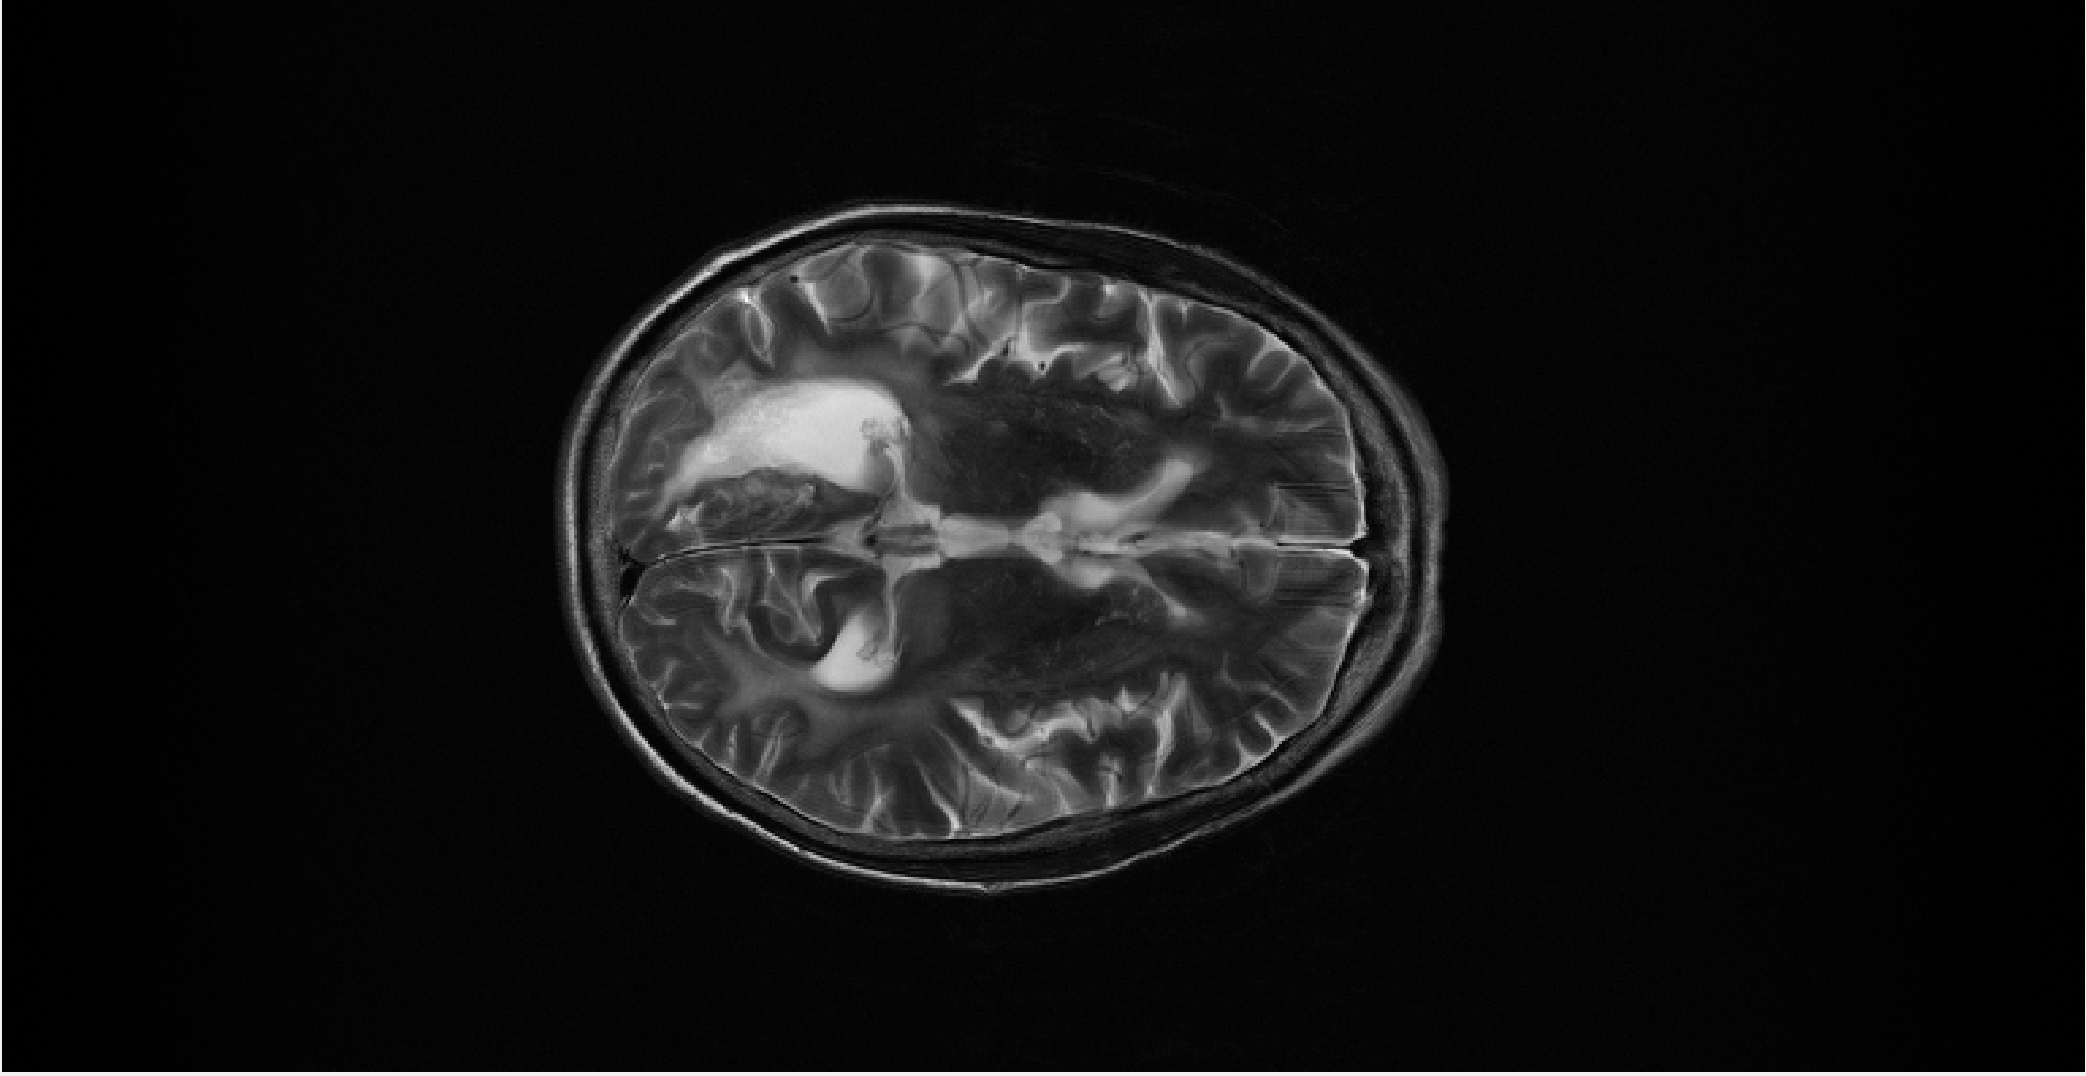
\includegraphics[scale=0.3]{./image/1.jpg}
	\caption{SMS}
\end{figure}
\begin{figure}[ht]
	\centering
	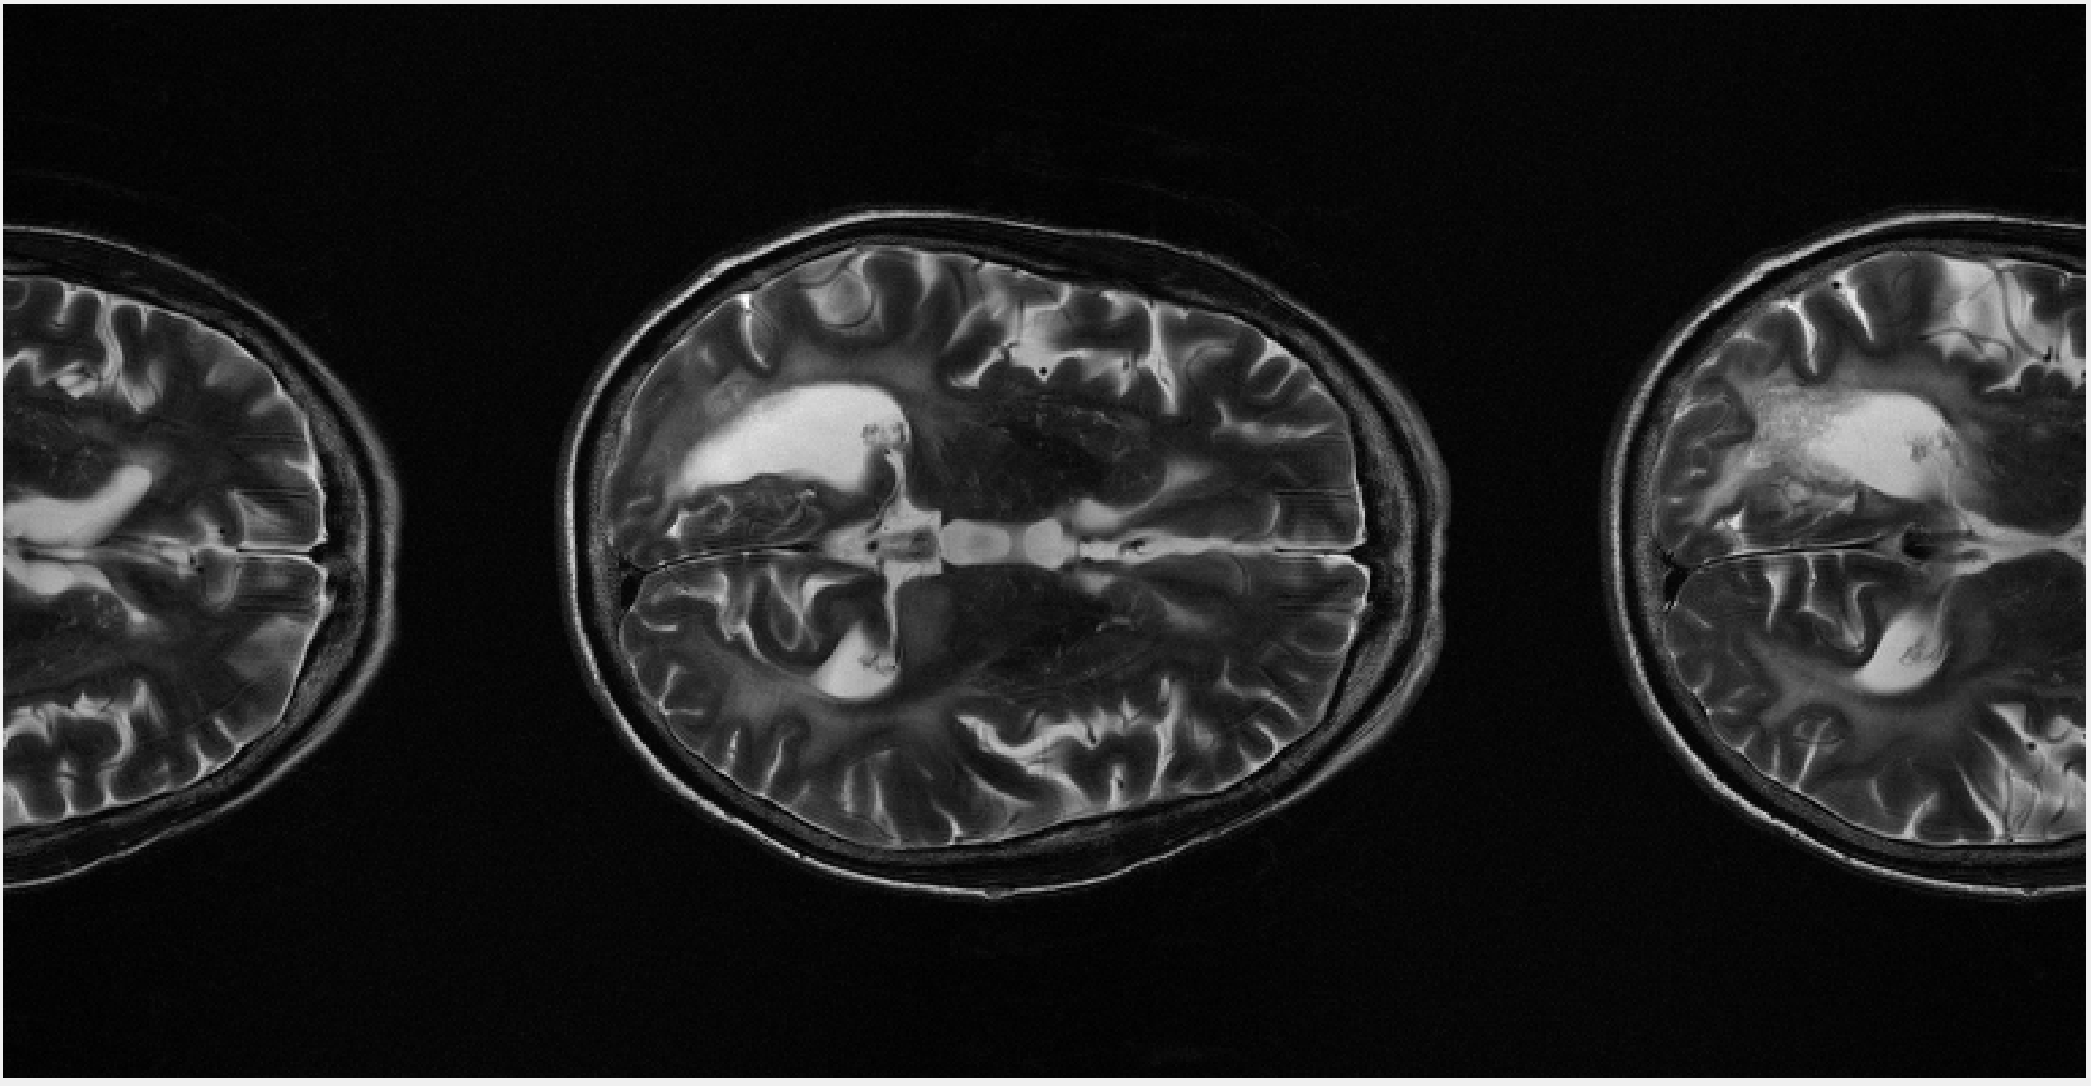
\includegraphics[scale=0.3]{./image/2.jpg}
	\caption{CAIPIRINHA SMS(0 $\pi$)}
\end{figure}
\par 基于CAIPIRINHA技术采集得到的SMS数据,传统的重建方法有SENSE/GRAPPA\cite{blaimer2006accelerated}, slice-GRAPPA(SG)\cite{setsompop2012blipped}等。SENSE/GRAPPA方法结合SENSE和GRAPPA的优势,将SMS重建问题分解成可以使用常规的一维GRAPPA解决的问题,SENSE/GRAPPA处理流程如图3所示。此时有同时激发的切片数量$N_s=2$,首先将两张切片的低分辨率图像沿着相位编码(PE)方向进行拼接,之后将得到的扩展图像矩阵进行傅里叶变换得到扩展的k-空间数据,之后使用传统GRAPPA算法计算用以重建的kernel,最后对SMS叠加的k-空间数据使用GRAPPA算法进行重建,即可以得到两张重建切片图像。
\par Slice-GRAPPA算法的处理流程如图4所示,其算法思想总体与单个切片的GRAPPA类似,但是它为每一个切片都会估计出一组kernel,而且与传统的GRAPPA内核对获取的k-空间数据进行操作以填充缺失的行不同,slice-GRAPPA内核为给定切片的每个线圈创建一组全新的k-空间数据。但是SG算法对不同层混叠后出现的伪影处理仍不够具有鲁棒性,因此在文\cite{cauley2014interslice}中提出了Split slice-GRAPPA(SP-SG),作者通过使用一个新的核拟合函数,得到了更具有鲁棒性的kernel,因此可以重建出质量较高的切片图像。文章\cite{hashemizadehkolowri2020coil}进一步优化了kernel的拟合函数,提出coil-combined split slice-GRAPPA(CG-SSG)。文\cite{hashemizadehkolowri2021simultaneous}基于SP-SG算法,并且结合图像域正则化的方法,提出了regularized image domain split slice-GRAPPA(RI-SSG),作者使用了具有显式灵敏度信息的SMS正向模型,并且对多切片图像进行TV正则化,最后在最小二乘的意义下求解模型。
\begin{figure}[ht]
	\centering
	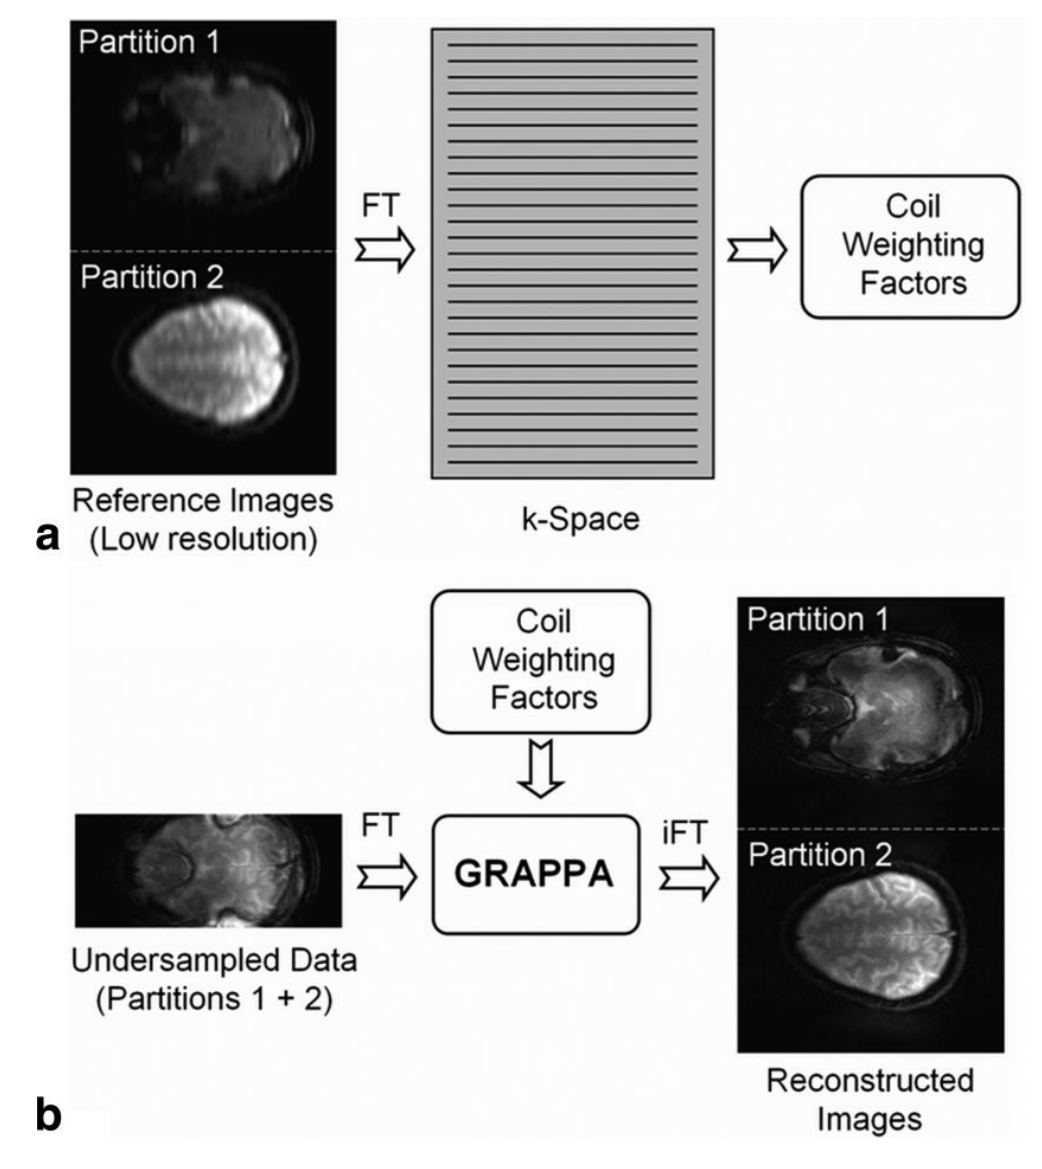
\includegraphics[scale=0.7]{./image/3.jpg}
	\caption{SENSE/GRAPPA}
\end{figure}
\begin{figure}[ht]
	\centering
	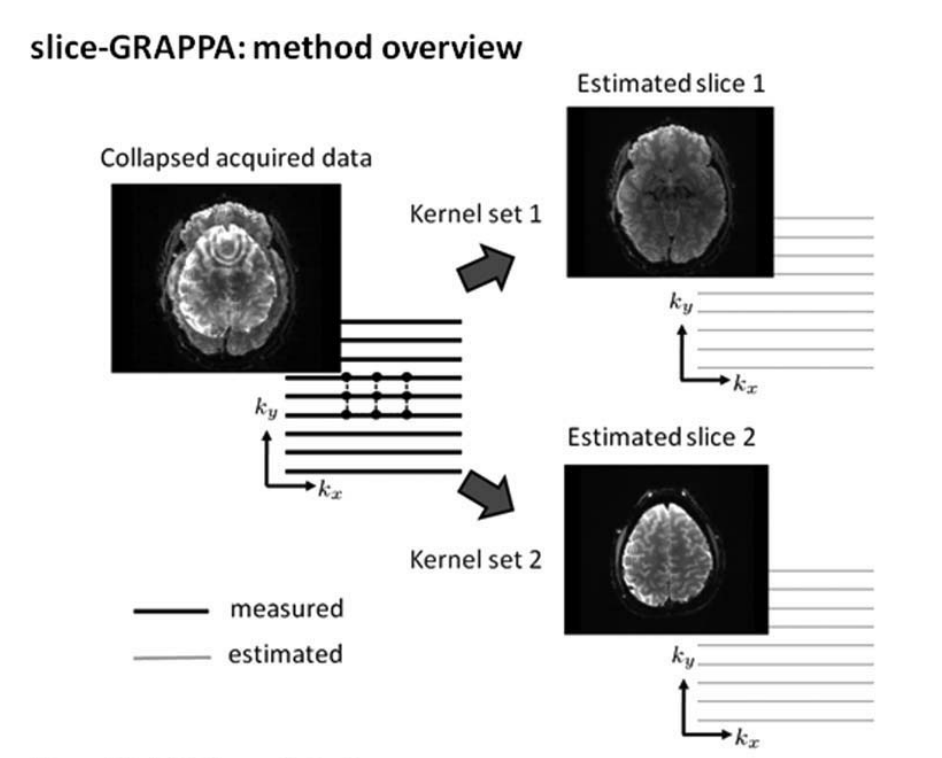
\includegraphics[scale=0.75]{./image/4.jpg}
	\caption{slice-GRAPPA}
\end{figure}
\newpage
\bibliographystyle{IEEEtran}
\bibliography{reference}
	
\end{document}